\chapter{Machine learning model specifications}
\label{chap:model}

\par Creating and training a model from scratch requires a lot of resources in terms of hardware and data, even with smaller models in order to achieve high performance, so in order to ensure good results I will utilize transfer learning with a pretrained MobileNet architecture.

\section{MobileNet specifications}
\label{sec:modelsec1}

\par The used model is downloaded from the TensorFlow Model Garden \cite{modelGarden}, specifically the ssd-mobilenet-v2-fpnlite-320x320-coco version. The ssd, meaning single shot detector, is an architecture which uses the MobileNet model as its base. Fpn means feature map network, which is a method to extract information from multiple resolution levels in the image and perform the object detection on those. Coco is the name of the dataset on which the model is initially trained and the 320x320 means the image resolution for training.

\subsection{Model specifications}
\label{sec:modelsec1subsec1}

\par The architecture being a single shot detector means that one pass through is enough for predicting the objects and their bounding boxes \cite{ssd}.

\begin{figure}
    \centering
    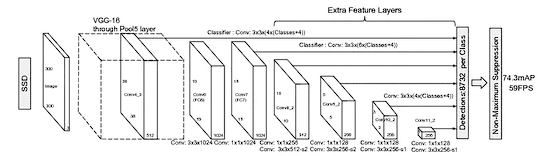
\includegraphics[width=0.5\linewidth]{figures/SSD.png}
    \caption{Architectural diagram of the SSD MobileNet model \cite{ssd}}
    \label{fig:ssd}
\end{figure}

\par In figure \ref{fig:ssd} we can see the overall architecture of a general ssd fpn model. In the case of this application the first few convolutional layers, the deep learning backbone, is replaced with the MobileNet architectures first few layer, which have been discussed in section \ref{subsec:relatedsec2subsec3}. The following few convolutional layers are the feature map network part. In this section the features processed by the machine learning model are made smaller and smaller, with every one of them having a connection to the prediction layer, hence enabling the architecture to learn with different ratios.
\par The predictions are done with help of 3x3xp kernels, where p is the number of channels in the feature map, which produce category scores or shape offsets for the bounding boxes. In the end filters are used at each cell in the feature maps to calculate 4 offsets relative to specified default bounding boxes \cite{ssd}.

\subsection{Original dataset}
\label{sec:modelsec1subsec2}

\par The model was pretrained on the COCO dataset, which contains around two hundred thousand labeled object in around 80 different categories, specifically made for the purposes of object detection by a team of researchers \cite{coco}.

\subsection{Model output}
\label{sec:modelsec1subsec3}

\par This architecture outputs a number of values regarding bounding boxes in raw and relative, value between 0 and 1, form and the predicted classes with their probabilities. In the case of the application three values are the most important: the class index, the prediction confidence and the relative bounding boxes. The confidence and index are needed for all hand gestures, while the box coordinate values are used when calculating the pixel positions for drawing.

\section{Data}
\label{sec:modelsec2}

\par In order to have creative freedom over the hand gestures, a custom dataset was made by me with five hand gestures and 20 pictures each. Some examples can be seen in figure \ref{customDataset}. The images than were labeled by hand with labelimg tool \cite{labelImg} and transformed into TF records, which is a specific format for the tensorflow object-detection api when teaching models with the script provided by them \cite{tfRecords}.

\begin{figure}
    \centering
    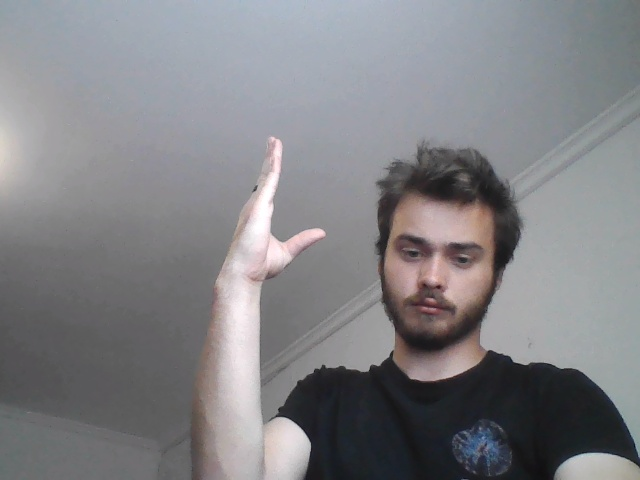
\includegraphics[width=0.22\linewidth]{figures/voiceup.jpg}
    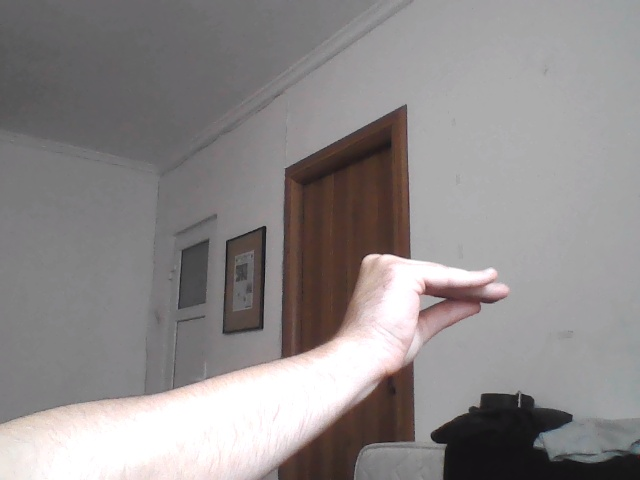
\includegraphics[width=0.22\linewidth]{figures/voicedown.jpg}
    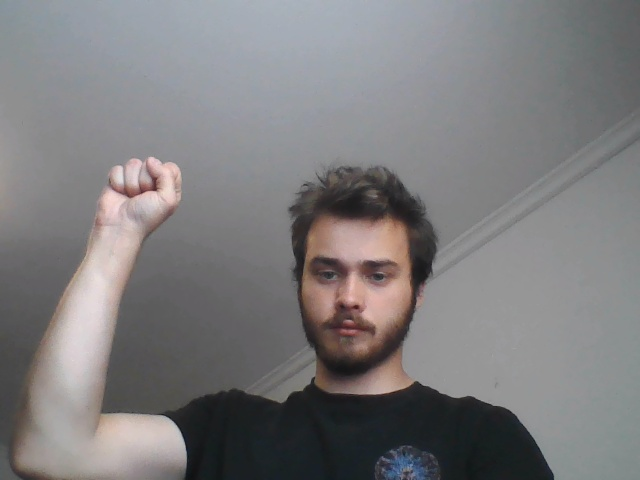
\includegraphics[width=0.22\linewidth]{figures/mute.jpg}
    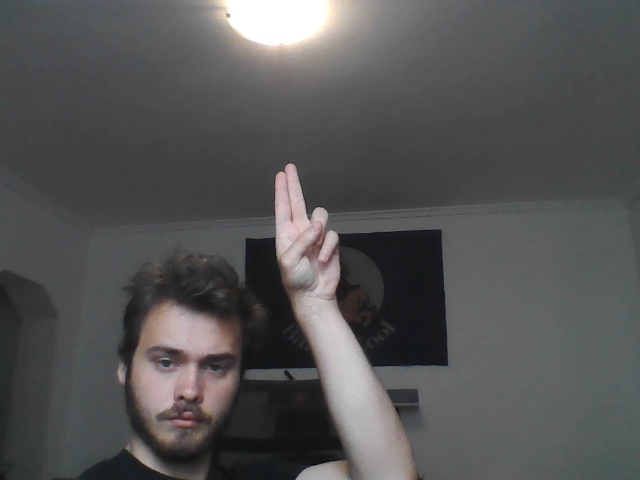
\includegraphics[width=0.22\linewidth]{figures/draw.jpg}
    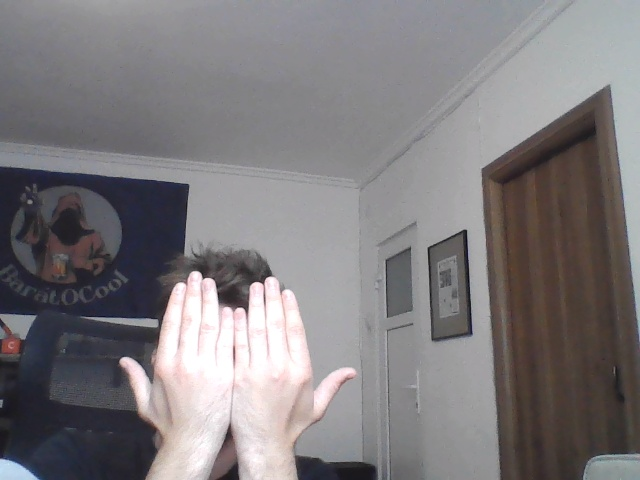
\includegraphics[width=0.22\linewidth]{figures/clear.jpg}
    \caption{Pictures for each functioning hand gesture in the dataset}
    \label{customDataset}
\end{figure}

\section{Training}
\label{sec:modelsec3}

\par The training of the model was done with the help of the provided script and configuration file by the tensorflow api \cite{trainingScript}. The configurations were personalized with the relevant paths to the label and record files and with the output path. The training was conducted with a batch size of 8 and 5 classes, decreasing learning rate and 20000 steps on an Nvidia 1660 Ti gpu.

\section{Metrics and running specifications}
\label{sec:modelsec4}

\par During training the learning rate slowly decreased in order to achieve a better approximations of the function as the model got closer to a local minimum, and the loss of the prediction have declined in a nice curve up until to a sufficient point, where it is low enough and the risk of over-fitting is not that high as can be seen in figure \ref{metrics}.

\begin{figure}
    \centering
    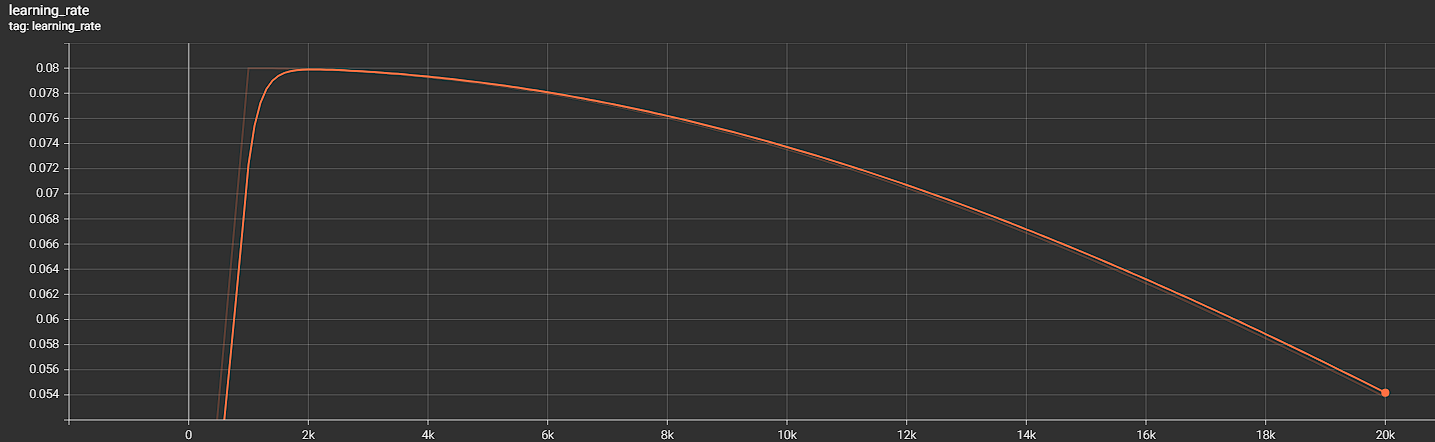
\includegraphics[width=0.4\linewidth]{figures/Learning-rate-graph.png}
    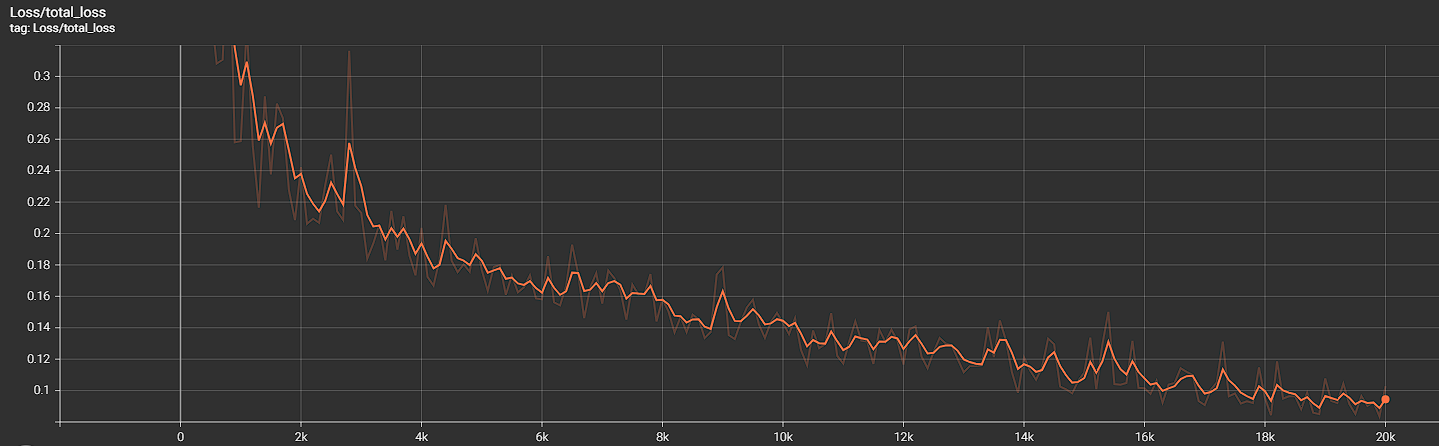
\includegraphics[width=0.4\linewidth]{figures/Loss-Graph.png}
    \caption{The changes of the learning rate and loss values throughout the training process}
    \label{metrics}
\end{figure}

\par As for the accuracy in real usage, the model can predict with around a 90 percent accuracy when the hand gesture features are visible. This means that the hands are not far enough from the camera, around 3 meters, that details can be barely visible, and an adequate light source is behind the camera.
\par For saving the application a script was provided by the api \cite{exportScript}, which exports the trained model in the format of the base tensorflow library, which makes the running of it easier in an application. To utilize the model the only thing that has to be done is to load it inside the application and add a batch layer to the image.